\subsection{\textbf{Exercise Sheet 1 Solution Spring 2025}}

\subsubsection{Q1.}
\begin{itemize}
  \item \textbf{Part A} - Suppose you have a sorted list of 128 names, and you’re searching through it using binary search. What’s the maximum number of steps it would take? 
  \textcolor{blue}{\textbf{Answer: 7}}.
  \item \textbf{Part B} - Suppose you double the size of the list. What’s the maximum number of steps now? 
  \textcolor{blue}{\textbf{Answer: 8}}.
\end{itemize}

\subsubsection{Q2.}
Give the run time for each of these scenarios in terms of Big O.
\begin{itemize}
  \item \textbf{Part A} - You have a name, and you want to find the person’s phone number in the phone book. 
  \textcolor{blue}{\textbf{Answer: $O(\log n)$}}.
  \item \textbf{Part B} - You have a phone number, and you want to find the person’s name in the phone book. (Hint: You’ll have to search through the whole book!) 
  \textcolor{blue}{\textbf{Answer: $O(n)$}}.
  \item \textbf{Part C} - You want to read the numbers of every person in the phone book. 
  \textcolor{blue}{\textbf{Answer: $O(n)$}}.
\end{itemize}

\subsubsection{Q3.}
What rule or criterion can be established to assess the overall time complexity of the selection statement, considering the functions $f(n)$ and $g(n)$ and the condition within the if statement?
\begin{lstlisting}[frame=single]
if 1 == 2:
    # something with O(f(n)) complexity
else:
    # something with O(g(n)) complexity
\end{lstlisting}

\textcolor{blue}{\textbf{Answer:}} The running time is $O(g(n))$. That is, the running time is that of the branch taken.

\subsubsection{Q4.}
In the context of Python, provide a big-O upper bound on the running time of the straightforward selection statement:

\begin{lstlisting}[frame=single]
while C:
    # Empty body
\end{lstlisting}

\textcolor{blue}{\textbf{Answer:}} If the condition 'C' evaluates to false, the running time of the while-loop is $O(1)$. In the case where the condition is true, the while-loop executes indefinitely, and the running time is undefined.

\subsubsection{Q5.}
Given a list of $n$ numbers, create a straightforward Python function \texttt{has\_duplicates} to determine if there are any duplicate elements in the array. Additionally, calculate the time and space complexity for the worst-case scenario of your function.

\textcolor{blue}{\textbf{Answer:}} In the worst case, the loop runs $n$ times, and the check inside it takes $O(n)$ time. Therefore, the overall time complexity is $O(n^2)$. In the worst case, if there are no duplicates, the \texttt{seen\_elements} list will store all $n$ elements of the input list. Therefore, the space complexity is $O(n)$.

\subsubsection{Q6. Merge Sort}
Use Merge Sort to sort the given list $[9, 7, 5, 11, 12, 2, 14, 3, 10, 6]$. Show the steps.\\
% \usetikzlibrary{shapes.multipart}

% \tikzset{block/.style={
%         font=\sffamily,
%         draw=black,
%         thin,
%         fill=pink!50,
%         rectangle split,
%         rectangle split horizontal,
%         rectangle split parts=#1,
%         outer sep=0pt},
%         %
%         gblock/.style={
%             block,
%             rectangle split parts=#1,
%             fill=green!30}
%         }


% \def\lvld{1.2}                  % Choose level distance
% \pgfmathsetmacro\shft{-6*\lvld} % Calculate the yshift for the green tree

% \begin{tikzpicture}[level distance=\lvld cm,
%   level 1/.style={sibling distance=4cm},
%   level 2/.style={sibling distance=2cm},
%   level 3/.style={sibling distance=1cm},
%   edgedown/.style={edge from parent/.style={draw=red,thick,-latex}},
%   edgeup/.style={edge from parent/.style={draw=green!50!black,thick,latex-}}
%   ]

% % GREEN TREE (drawn first to let the middle line filled in pink)

% \node[gblock=7,yshift=\shft cm] (A') {3 \nodepart{two} 9 \nodepart{three} 10 \nodepart{four} 27 \nodepart{five} 39 \nodepart{six}43 \nodepart{seven}82}
% [grow=up,edgeup]
% child {node[gblock=3] (B2') {9 \nodepart{two} 10 \nodepart{three} 82}
% child {node[gblock=1] (C4') {10}
% child {node[gblock=1] (D7') {10}}
% }
% child {node[gblock=2] (C2') {9 \nodepart{two} 82}
% child {node[gblock=1] (D3') {82}}
% child {node[gblock=1] (D4') {9}}
% }
% }
% child {node[gblock=4] (B1') {3 \nodepart{two} 27 \nodepart{three} 39 \nodepart{four} 43}
% child {node[gblock=2] (C3') {3 \nodepart{two} 43}
% child {node[gblock=1] (D5') {3}}
% child {node[gblock=1] (D6') {43}}
% }
% child {node[gblock=2] (C1') {27 \nodepart{two} 39}
% child {node[gblock=1] (D1') {27}}
% child {node[gblock=1] (D2') {39}}
% }
% };


% % PINK TREE

% \node[block=7] (A) {39 \nodepart{two} 27 \nodepart{three} 43 \nodepart{four} 3 \nodepart{five} 9 \nodepart{six}82 \nodepart{seven}10}
% [grow=down,edgedown]
% child {node[block=4] (B1) {39 \nodepart{two} 27 \nodepart{three} 43 \nodepart{four} 3}
% child {node[block=2] (C1) {39 \nodepart{two} 27}
% child {node[block=1] (D1) {39}}
% child {node[block=1] (D2) {27}}
% }
% child {node[block=2] (C2) {43 \nodepart{two} 3}
% child {node[block=1] (D3) {43}}
% child {node[block=1] (D4) {3}}
% }
% }
% child {node[block=3] (B2) {9 \nodepart{two} 82 \nodepart{three} 10}
% child {node[block=2] (C3) {9 \nodepart{two} 82}
% child {node[block=1] (D5) {9}}
% child {node[block=1] (D6) {82}}
% }
% child {node[block=1] (C4) {10}
% child {node[block=1] (D7) {10}}
% }
% };
% \end{tikzpicture}

\begin{center}
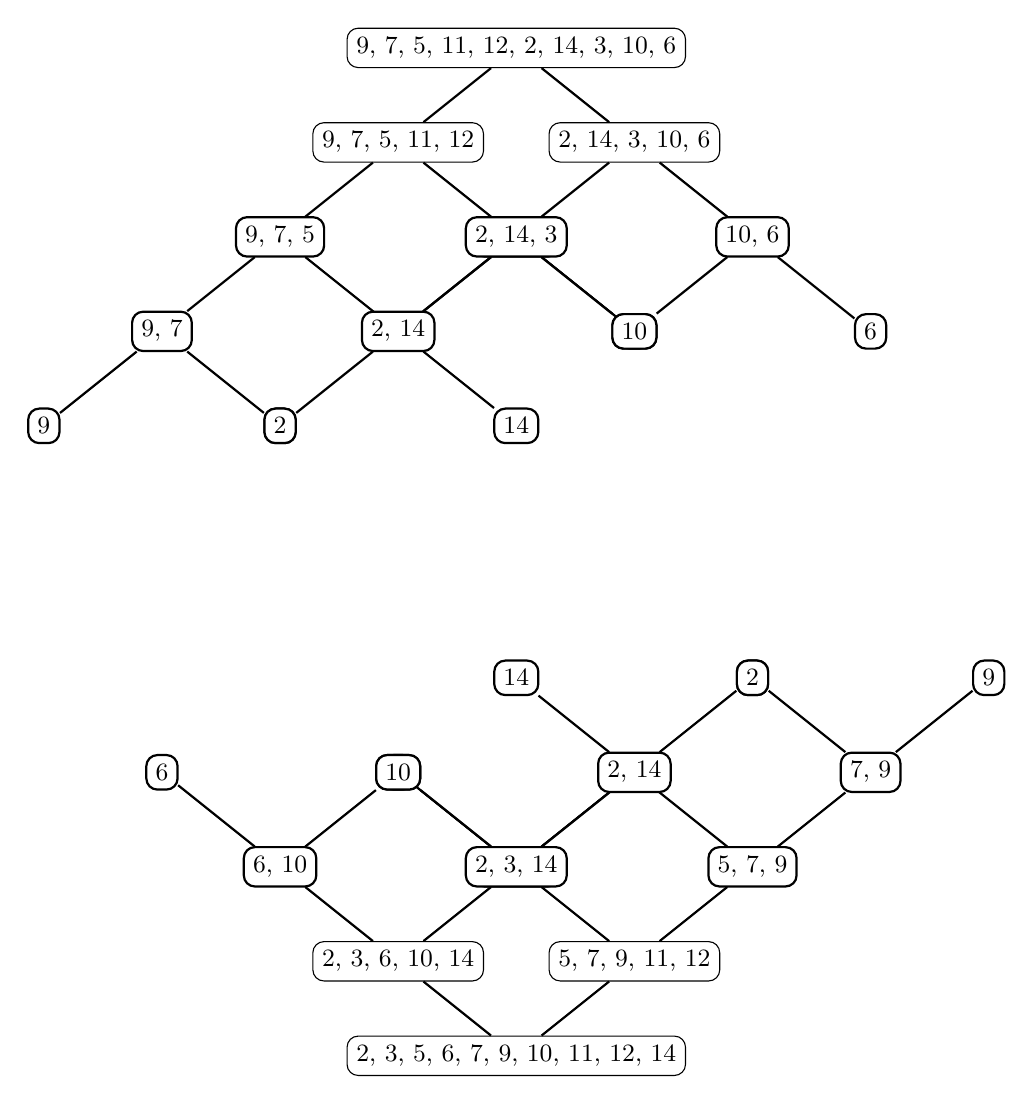
\begin{tikzpicture}[
  grow=down,
  level distance=1.2cm,
  sibling distance=3cm,
  every node/.style={draw=black, rounded corners, fill=white, font=\small, align=center},
  edge from parent/.style={draw, thick}
  ]

% SPLIT tree
\node {9, 7, 5, 11, 12, 2, 14, 3, 10, 6}
  child {
    node {9, 7, 5, 11, 12}
    child {
      node {9, 7, 5}
      child {
        node {9, 7}
        child {node {9}}
        child {node {7}}
      }
      child {node {5}}
    }
    child {
      node {11, 12}
      child {node {11}}
      child {node {12}}
    }
  }
  child {
    node {2, 14, 3, 10, 6}
    child {
      node {2, 14, 3}
      child {
        node {2, 14}
        child {node {2}}
        child {node {14}}
      }
      child {node {3}}
    }
    child {
      node {10, 6}
      child {node {10}}
      child {node {6}}
    }
  };

% MERGE tree (rotated upside down)
\begin{scope}[yshift=-12.8cm, rotate=0, grow=up, level distance=1.2cm]
\node {2, 3, 5, 6, 7, 9, 10, 11, 12, 14}
  child {
    node {5, 7, 9, 11, 12}
    child {
      node {5, 7, 9}
      child {
        node {7, 9}
        child {node {9}}
        child {node {7}}
      }
      child {node {5}}
    }
    child {
      node {11, 12}
      child {node {11}}
      child {node {12}}
    }
  }
  child {
    node {2, 3, 6, 10, 14}
    child {
      node {2, 3, 14}
      child {
        node {2, 14}
        child {node {2}}
        child {node {14}}
      }
      child {node {3}}
    }
    child {
      node {6, 10}
      child {node {10}}
      child {node {6}}
    }
  };
\end{scope}
\end{tikzpicture}
\end{center}

\textcolor{blue}{\textbf{Answer:}}\\

\textit{Hand-drawn tree not included here. For full documentation, the merge sort tree would need to be recreated using TikZ or similar packages.}\\

Final sorted list: $[2, 3, 5, 6, 7, 9, 10, 11, 12, 14]$

\subsubsection{Q7. Bubble Sort}
Use Bubble Sort to sort the given list $[9, 7, 5, 11, 12, 2, 14, 3, 10, 6]$. Show the steps.

\textcolor{blue}{\textbf{Answer:}} Compare each pair of adjacent elements, swapping them if they are in the wrong order. After the first pass, the largest element will be bubbled to the end of the list.

\begin{itemize}
    \item Initial list: $[9, 7, 5, 11, 12, 2, 14, 3, 10, 6]$
    \item After the first pass: $[7, 5, 9, 11, 2, 12, 3, 10, 6, 14]$
    \item Repeat the same process for the remaining elements except the last one.\\
          $[7, 5, 9, 11, 2, 12, 3, 10, 6, 14]$
    \item After the second pass: $[5, 7, 9, 2, 11, 3, 10, 6, 12, 14]$\\
          Repeat the process again.\\
          $[5, 7, 9, 2, 11, 3, 10, 6, 12, 14]$
    \item After the third pass: $[5, 7, 2, 9, 3, 10, 6, 11, 12, 14]$\\
          Repeat the process.\\
          $[5, 7, 2, 9, 3, 10, 6, 11, 12, 14]$
    \item After the fourth pass: $[5, 2, 7, 3, 9, 6, 10, 11, 12, 14]$\\
          Repeat the process.\\
          $[5, 2, 7, 3, 9, 6, 10, 11, 12, 14]$
    \item After the fifth pass: $[2, 5, 3, 7, 6, 9, 10, 11, 12, 14]$
    \item $\ldots$
    \item After the 9$^{\text{th}}$ ($n-1$) pass: $[2, 3, 5, 6, 7, 9, 10, 11, 12, 14]$
\end{itemize}

\subsubsection{Q8. [Linear and Binary Search]}
You are given a sorted array of integers: \\
$E = [2, 5, 8, 11, 14, 17, 20, 23, 26]$. Use linear search and binary search to find the index of the element 17 in the array. Show each step of the process.

\textcolor{blue}{\textbf{Answer:}}

\textbf{Linear Search:}
\begin{itemize}
    \item Compare 17 with $E[0]$ (2) -- not a match.
    \item Compare 17 with $E[1]$ (5) -- not a match.
    \item Compare 17 with $E[2]$ (8) -- not a match.
    \item Compare 17 with $E[3]$ (11) -- not a match.
    \item Compare 17 with $E[4]$ (14) -- not a match.
    \item Compare 17 with $E[5]$ (17) -- match found.
\end{itemize}
\textbf{Result:} The index of 17 is 5.

\textbf{Binary Search:}
\begin{itemize}
    \item Set $l = 0$, $r = 8$.
    \item Calculate $mid = (0 + 8) \div 2 = 4$.
    \item Compare 17 with $E[4]$ (14) -- 17 is greater, so narrow to upper half.
    \item Set $l = 4 + 1 = 5$, $r = 8$.
    \item Calculate $mid = (5 + 8) \div 2 = 6$.
    \item Compare 17 with $E[6]$ (20) -- 17 is less, so narrow to lower half.
    \item Set $l = 5$, $r = 6 - 1 = 5$.
    \item Calculate $mid = (5 + 5) \div 2 = 5$.
    \item Compare 17 with $E[5]$ (17) -- match found.
\end{itemize}


\textbf{Result:} The index of 17 is 5.